The calorimeter response to particles is not linear and it is not straightforward to translate the measured jet energy
to that of the original parton.
In data, these deviations are driven by the non-uniformity and non-linearity of the calorimeter response,
while in Monte Carlo simulation, the corrections ensure a posteriori the agreement with the observed data.
Furthermore, contributions from \pileup{} events or detector noise may bias the measurement of the jet energy.
To this end, a calibration of the reconstructed jet is performed by applying a series of corrections on the measured jet energy,
collectively referred to as Jet Energy Scale corrections (JES).
%% This class of corrections represents an important source of systematic uncertainty in the analyses with a multi-jet final state.

\begin{figure}
\centering
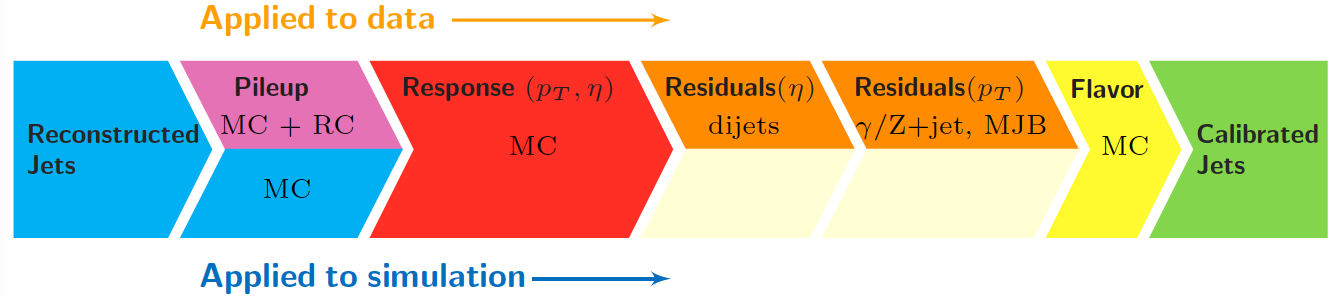
\includegraphics[width=.8\textwidth]{JEC_levels.png}
\caption{Overview of the jet energy calibration procedure follwed in data and simulation~\cite{CMS-JME-13-004}.}
\label{fig:JECoverview}
\end{figure}

%% The corrections, parametrized as function of \pt and $\eta$ of the jets, are applied following the standard procedure used by most of the CMS analyses \cite{CMS:JEC_2011, CMS-DP-2016-020, CMS-DP-2021-033}.

\paragraph{Jet energy scale\\}
The JES corrections are calculated in the form of a multiplicative factor on the four-momentum of the measured jet,
in order to match the measured energy of each jet to its true energy at the generator level.
The measured jet transverse momentum response is defined as the ratio of the measured jet \pt at the reconstruction step to the generated jet at particle level.
%% These corrections and the corresponding uncertainties are provided centrally by the CMS JetMet group

\Pileup{} offset corrections account for the measured energy of the jet in excess due to
the presence of in-time (IT) and out-of-time (OOT) \pileup{}
%% They are derived from the simulation of QCD multi-jet events processed with or without \pileup{} overlay
and they are applied to both data and MC samples.

Simulated response corrections compensate for the non-linear response in \pt and pseudorapidity
from the calorimeters and tracker coverage and they are parametrized as a function of these jet kinematic variables.

Residual data to Monte Carlo corrections are applied to improve the agreement as a function of the jet $\eta$ and \pt.
The absolute scale of the measured jet \pt response is corrected in data using multi-jet and Drell-Yan plus jets events,
which benefit from the high precision measurement of the \PZ boson and the photon energy in the ECAL.
The residual $\eta$ correction is derived in di-jet events exploiting the \pt imbalance of the di-jet system.

\paragraph{Jet energy resolution\\}
Jet Energy Resolution (JER) corrections introduce a dose of smearing in the simulated jet \pt spectrum
to compensate for data-to-simulation differences due to detector resolution effects.
They are determined in $\PGg/\PZ$ + jets events by fitting the residual of the \pt distribution to a
double-sided Crystall Ball function.
This accounts for a gaussian core due to statistical fluctuations in the deposited energy,
while the tails account for effects such as inactive areas, neutrino emissions in heavy flavour in-flight decays
or punch-though of hadrons beyond the end of the calorimeter.
